\begin{EXO}{Tableaux et diagrammes}{5I13}
Laurent, le \acc{cuisinier d'un collège}, souhaite \acc{étudier l'évolution} de sa consommation de carottes. 

Il a réalisé le \acc{tableau} suivant à la main et souhaite représenter cette série statistique par un \acc{diagramme}
afin de visualiser plus rapidement cette évolution.
% Tableau des données
\begin{center}
\vspace{-0.2cm}\begin{tcbtab}{c|c|c|c|c|c|c|c|c|c|c}%

\cellcolor{\currentTableColbackTitleColor}{\color{\currentTableColTitleColor} \textbf{Mois}} & \textbf{Sept.} & \textbf{Oct.} & \textbf{Nov.} & \textbf{Déc.} & \textbf{Janv.} & \textbf{Févr.} & \textbf{Mars} & \textbf{Avril} & \textbf{Mai} & \textbf{Juin} \\
\hline
\cellcolor{\currentTableColbackTitleColor}{\color{\currentTableColTitleColor} \textbf{Masse en kg}} & 15 & 20 & 26 & 18 & 20 & 35 & 28 & 18 & 12 & 6 \\
\end{tcbtab}
\end{center}
\vspace{-0.25cm}\begin{MultiColonnes}{3}
    \tcbitem  \infotcbitempoint{4}[-0.65][-1cm]On cherche à réaliser le graphique ci-contre.
    \begin{tcbenumerate}
        \tcbitem \acc{Ouvre} une feuille de calcul et reproduis le tableau ci-dessus.

        \tcbitem \acc{Après} avoir sélectionné les cellules, clique sur l'icône indiquée par la flèche sur la capture d'écran.
        \vspace{-0.35cm}\begin{center}
\includegraphics[width=0.6\textwidth]{images/libreoffice_icone_diagramme.png}
\end{center}
    \end{tcbenumerate}
\tcbitem[raster multicolumn=2] \begin{center}
% Diagramme en barres avec TikZ/PGFPlots
% Diagramme en barres amélioré avec TikZ/PGFPlots
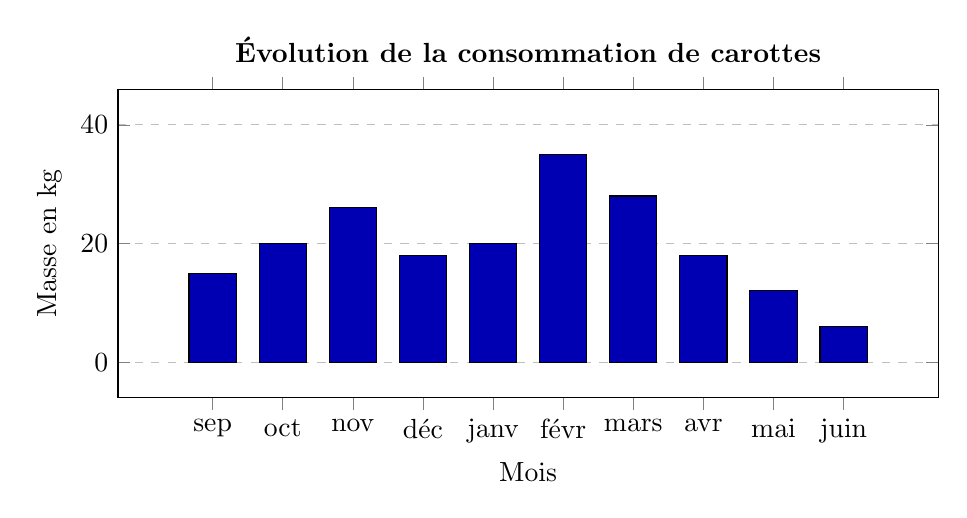
\begin{tikzpicture}
\begin{axis}[
    title={Évolution de la consommation de carottes},
    title style={font=\bfseries},
    xlabel={Mois},
    ylabel={Masse en kg},
    symbolic x coords={sep, oct, nov, déc, janv, févr, mars, avr, mai, juin},
    xtick=data,
    ymin=0,
    ymax=40,
    width=12cm,
    height=5.5cm,
    bar width=0.6cm,
    enlargelimits=0.15,
    ymajorgrids=true,
    grid style=dashed,
    legend pos=north west,
    ybar,
]
%options désactivées :
%    nodes near coords,
%    nodes near coords align={vertical},
\addplot[fill=blue!70!black] coordinates {
    (sep,15) (oct,20) (nov,26) (déc,18) (janv,20) (févr,35) (mars,28) (avr,18) (mai,12) (juin,6)
};
\end{axis}
\end{tikzpicture}
\end{center}
\end{MultiColonnes}
\vspace{-0.5cm}\begin{MultiColonnes}{3}
    \tcbitem \begin{tcbenumerate}[1][3] 
        \tcbitem \infotcbitempoint{2}[0.15]\acc{Dans} la fenêtre 
        
        qui s'ouvre, choisis \encadrer{ Colonne }, puis, dans le menu de gauche \encadrer{ 4. Éléments du diagramme }
    \end{tcbenumerate}
    \tcbitem[raster multicolumn=2,halign=center,valign=center] \includegraphics[width=0.8\textwidth]{images/libreoffice_fenetre_choix_diagramme.png}
\end{MultiColonnes}
\vspace{-0.25cm}\begin{tcbenumerate}[1][4]
\tcbitem \infotcbitempoint{3}[0.1]\acc{Saisis} :

\begin{MultiColonnes}{3}
    \tcbitem[raster multicolumn=2] \begin{itemize}[label=$\bullet$]
  \item dans Titre :  \encadrer{Évolution de la consommation de carottes} .
  \item dans Axe X :  \encadrer{Mois} .
  \item dans Axe Y :  \encadrer{Masse en kg} .
\end{itemize}

Décoche la case \encadrer{ Afficher la légende }, puis clique sur \encadrer{ Terminer }.

    \tcbitem \begin{center}
\includegraphics[width=\textwidth]{images/libreoffice_parametres_diagramme.png}
\end{center}
\end{MultiColonnes}
\tcbitem \infotcbitempoint{2}[0.1]\acc{Encadrer le titre sur ton graphique}. 

\begin{MultiColonnes}{3}
    \tcbitem[raster multicolumn=2] \begin{itemize}[label=$\bullet$] 
        \item Clique sur le titre pour l'\acc{activer}. 
        \item \acc{Effectue un clic droit} avec la souris. Dans le menu qui apparaît, clique sur \encadrer{ Formater le titre }. 
        \item Dans l'onglet \encadrer{ Bordure }, pour \encadrer{ Style }, choisis \encadrer{ Continu }. 
    \end{itemize}
    \tcbitem \begin{center}
\includegraphics[width=\textwidth]{images/libreoffice_alignement_axe.png}
\end{center}
\end{MultiColonnes}
\tcbitem \infotcbitempoint{4}[-0.65]\acc{Ouvre le menu} \encadrer{ Formater le titre } pour \encadrer{ Masse en kg }. Dans l'onglet \encadrer{ Alignement }, tourne le petit carré jusqu'à ce que l'angle soit égal à 0 degré. 
\end{tcbenumerate}

\end{EXO}